%% generato automaticamente da tools/build_tex.py --- non modificare
\chapter{Oscillazioni a frequenza crescente}
\label{cap:cost2}
\quaderno{cost\textasciicircum{}2.dfw}{24 Jun 2010}{22}

Giugno 2010. Ventidue espressioni su $\cos(t^2)$ e $\sin(t^2)$: funzioni che oscillano sempre più rapidamente man mano che ci si allontana dall'origine, e i cui integrali non si esprimono con funzioni elementari. Sono gli integrali di Fresnel, e il quaderno li incontra senza chiamarli per nome. La sezione finale, però, arriva a un risultato esatto e notevole.

\section{Le funzioni e le loro derivate}

Le prime dodici righe stabiliscono il comportamento sotto derivazione, che è ordinato e prevedibile.

\begin{espr}{1}{User}{}
\[
\sin\!\left(t^{2}\right)
\]
\end{espr}
Il seno di un quadrato: oscilla sempre più rapidamente al crescere di $|t|$.

\begin{espr}{2}{User}{}
\[
\cos\!\left(t^{2}\right)
\]
\end{espr}
Il coseno corrispondente.

\begin{espr}{3}{User}{}
\[
\sin^{2}\!\left(t^{2}\right)
\]
\end{espr}
Il quadrato del primo.

\begin{espr}{4}{User}{}
\[
\cos^{2}\!\left(t^{2}\right)
\]
\end{espr}
E del secondo. La loro somma vale identicamente uno.

\begin{espr}{5}{Dif(\#2,t)}{}
\[
\frac{\mathrm{d}}{\mathrm{d}t}\!\left[\cos\!\left(t^{2}\right)\right]
\]
\end{espr}
Si deriva il coseno.

\begin{espr}{6}{Simp(Dif(\#2,t))}{}
\[
-2\, t\, \sin\!\left(t^{2}\right)
\]
\end{espr}
Il risultato: compare il fattore $2t$, responsabile dell'infittirsi delle oscillazioni.

\begin{espr}{7}{Dif(\#1,t)}{}
\[
\frac{\mathrm{d}}{\mathrm{d}t}\!\left[\sin\!\left(t^{2}\right)\right]
\]
\end{espr}
Si deriva il seno.

\begin{espr}{8}{Simp(Dif(\#1,t))}{}
\[
2\, t\, \cos\!\left(t^{2}\right)
\]
\end{espr}
Con il segno opposto, come atteso.

\begin{espr}{9}{Dif(\#6,t)}{}
\[
\frac{\mathrm{d}}{\mathrm{d}t}\!\left[-2\, t\, \sin\!\left(t^{2}\right)\right]
\]
\end{espr}
Seconda derivata del coseno.

\begin{espr}{10}{Simp(Dif(\#6,t))}{}
\[
-4\, t^{2}\, \cos\!\left(t^{2}\right) - 2\, \sin\!\left(t^{2}\right)
\]
\end{espr}
Compaiono un termine in $t^2$ e uno costante.

\begin{espr}{11}{Dif(\#8,t)}{}
\[
\frac{\mathrm{d}}{\mathrm{d}t}\!\left[2\, t\, \cos\!\left(t^{2}\right)\right]
\]
\end{espr}
Seconda derivata del seno.

\begin{espr}{12}{Simp(Dif(\#8,t))}{}
\[
2\, \cos\!\left(t^{2}\right) - 4\, t^{2}\, \sin\!\left(t^{2}\right)
\]
\end{espr}
La struttura è la stessa, con le funzioni scambiate.


Derivando una volta compare il fattore $2t$, derivando due volte compaiono un termine in $t^2$ e uno costante. Il punto rilevante è che le due funzioni si scambiano a ogni derivazione ma il fattore $2t$ cresce: è questo che rende l'oscillazione sempre più fitta e che impedisce alle primitive di essere elementari.

\section{Le combinazioni e i loro integrali}

Il quaderno costruisce la semisomma e la semidifferenza delle due funzioni e ne chiede le primitive.

\begin{espr}{13}{User}{}
\[
\frac{\cos\!\left(t^{2}\right) + \sin\!\left(t^{2}\right)}{2}
\]
\end{espr}
La semisomma delle due funzioni.

\begin{espr}{14}{Int(\#13,t)}{}
\[
\int \frac{\cos\!\left(t^{2}\right) + \sin\!\left(t^{2}\right)}{2} \,\mathrm{d}t
\]
\end{espr}
Il suo integrale indefinito, che Derive lascia indicato.

\begin{espr}{15}{User}{}
\[
\int \frac{\cos\!\left(t^{2}\right) - \sin\!\left(t^{2}\right)}{2} \,\mathrm{d}t
\]
\end{espr}
La semidifferenza, con lo stesso trattamento.

\begin{espr}{16}{Int(\#2,t)}{}
\[
\int \cos\!\left(t^{2}\right) \,\mathrm{d}t
\]
\end{espr}
L'integrale del solo coseno: è l'integrale di Fresnel $C$.

\begin{espr}{17}{Int(\#1,t)}{}
\[
\int \sin\!\left(t^{2}\right) \,\mathrm{d}t
\]
\end{espr}
E quello del solo seno: l'integrale di Fresnel $S$. Nessuno dei due è elementare.

\begin{figure}[htbp]
  \centering
  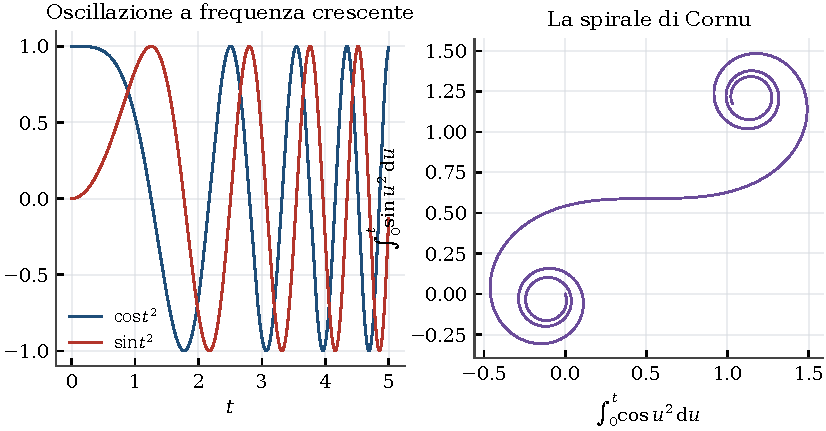
\includegraphics[width=0.86\linewidth]{../figures/fresnel.pdf}
  \caption{A sinistra le due funzioni: l'oscillazione si infittisce come $t$. A destra la curva che ha per coordinate i due integrali di Fresnel — la spirale di Cornu — i cui due punti limite sono le code convergenti dell'integrale improprio.}
  \label{fig:fresnel}
\end{figure}

Derive restituisce gli integrali senza valutarli, e fa bene: non esistono primitive elementari. Le funzioni $\int_0^t\cos u^2\,\mathrm{d}u$ e $\int_0^t\sin u^2\,\mathrm{d}u$ sono per definizione gli integrali di Fresnel, e la curva che si ottiene prendendole come coordinate di un punto è la spirale di Cornu — una delle curve più belle dell'analisi, e quella che descrive la diffrazione della luce da un bordo.

\section{L'integrale improprio}

L'ultima sezione introduce un parametro di frequenza e passa all'integrale su tutta la retta. Qui, dove la primitiva non esisteva, il valore esiste.

\begin{espr}{18}{User}{}
\[
\frac{\cos\!\left(\omega\, t^{2}\right) + \sin\!\left(\omega\, t^{2}\right)}{2}
\]
\end{espr}
Si introduce una frequenza $\omega$.

\begin{espr}{19}{User}{}
\[
\int_{-\infty}^{+\infty} \frac{\cos\!\left(\omega\, t^{2}\right) + \sin\!\left(\omega\, t^{2}\right)}{2} \,\mathrm{d}t
\]
\end{espr}
L'integrale su tutta la retta.

\begin{espr}{20}{Simp(\#19)}{}
\[
\frac{\sqrt{2}\, \sqrt{\pi}}{2\, \sqrt{\omega}}
\]
\end{espr}
Il valore esatto, $\sqrt{\pi/(2\omega)}$: l'integrale converge pur non essendo la funzione infinitesima all'infinito.

\begin{espr}{21}{User}{}
\[
\int_{-\infty}^{+\infty} \frac{t^{2}\, \left(\cos\!\left(\omega\, t^{2}\right) + \sin\!\left(\omega\, t^{2}\right)\right)}{2} \,\mathrm{d}t
\]
\end{espr}
Lo stesso integrale con un fattore $t^2$.

\begin{espr}{22}{Simp(\#21)}{}
\[
2\, \int_{0}^{\infty} \frac{t^{2}\, \cos\!\left(t^{2}\, \omega\right)}{2} + \frac{t^{2}\, \sin\!\left(t^{2}\, \omega\right)}{2} \,\mathrm{d}t
\]
\end{espr}
Derive lo riscrive sfruttando la parità ma non lo valuta: con quel fattore la cancellazione delle oscillazioni non basta più e l'integrale diverge.


Il risultato della riga $\#20$ è esatto e vale la pena di ricostruirlo. Gli integrali di Fresnel su tutta la semiretta valgono
\[
  \int_0^{+\infty}\cos\!\left(\omega t^2\right)\mathrm{d}t
  =\int_0^{+\infty}\sin\!\left(\omega t^2\right)\mathrm{d}t
  =\frac{1}{2}\sqrt{\frac{\pi}{2\omega}},
\]
e su tutta la retta valgono il doppio. La semisomma delle due dà dunque $\sqrt{\pi/(2\omega)}$, che è esattamente $\dfrac{\sqrt2\,\sqrt\pi}{2\sqrt\omega}$ come scritto.

È il fenomeno tipico degli integrali oscillanti: la funzione non tende a zero all'infinito e non è assolutamente integrabile, eppure l'integrale converge, perché le oscillazioni diventano così fitte che i contributi positivi e negativi si cancellano sempre meglio. La riga $\#21$ prova a spingersi oltre inserendo un fattore $t^2$, e lì la cancellazione non basta più: l'integrale diverge, e Derive si limita a riscriverlo sfruttando la parità, senza valutarlo.

\section*{In sintesi}
\addcontentsline{toc}{section}{In sintesi}

Ventidue righe che percorrono la distanza fra due situazioni opposte: una funzione le cui primitive non sono esprimibili con funzioni elementari, e il cui integrale su tutta la retta è invece una radice quadrata di $\pi$ scritta in tre simboli. Fra le due cose sta la spirale di Cornu, che il quaderno non disegna ma che le sue righe descrivono per intero.

